\paragraph{Protocol.} A preregistered rule picked the configuration on the validation split: two bands, discrepancy $\kappa=0.5$ and a GP length scale of 5\,d. We fixed five hypotheses. H1 says P is less often confidently wrong than B3 on unmodelled events. H2 says $P(h_0)$ ranks unmodelled events above modelled ones (AUROC $>0.5$). On supernovae, H3 says P is not more than 5 points more often confidently wrong than B3, and H5 says it is not more than 5 points less accurate. H4 says colour raises the AUROC over a single-band arm on the same events. Each hypothesis has to pass on all three noise seeds (stratified paired bootstrap, $10^4$ resamples). The test events (\RealNEvents: \RealNModeled\ supernovae, \RealNWithheld\ unmodelled) had already been used twice, in the retrospective analyses, so this causal run is a declared third look.

\paragraph{Results.} Table~\ref{tab:real} shows both versions side by side. With causal measurements, H1--H4 pass and H5 fails. Closed-world EIG was confidently wrong on \RealCCwWhBthree\ of real unmodelled transients (\RealRCwWhBthree\ retrospectively), the auction baseline B1 on \RealCCwWhBone, and P on \RealCCwWhP. P labelled \RealCFlagP\ of unmodelled events as unknown, with an AUROC of \RealCAuc\ (Fig.~\ref{fig:rocreal}).

\begin{table*}[t]
\centering\scriptsize
\caption{Real ZTF replay, preregistered test results per noise seed: estimate [95\% CI]; $^\times$ marks a criterion not met on that seed. CW: confident-wrong rate. $\Delta$: P minus B3, or the colour arm minus the single-band arm for H4. The causal version (v3) is this paper's result. The retrospective version (v2) let planners measure earlier epochs after later ones and is shown only for comparison.}
\label{tab:real}
\begin{tabular}{lll@{\hspace{4pt}}l}
\toprule
& Seed & Causal (v3) & Retrospective (v2) \\
\midrule
H1 $\Delta$CW unmod. & 1 & -0.49 [-0.60, -0.36] & -0.60 [-0.72, -0.49] \\
 & 2 & -0.42 [-0.55, -0.30] & -0.67 [-0.77, -0.56] \\
 & 3 & -0.36 [-0.48, -0.25] & -0.60 [-0.73, -0.48] \\
\addlinespace
H2 AUROC $P(h_0)$ & 1 & +0.81 [+0.76, +0.86] & +0.80 [+0.75, +0.85] \\
 & 2 & +0.81 [+0.76, +0.86] & +0.80 [+0.75, +0.85] \\
 & 3 & +0.79 [+0.73, +0.84] & +0.77 [+0.71, +0.82] \\
\addlinespace
H3 $\Delta$CW mod. & 1 & -0.05 [-0.09, -0.01] & +0.00 [-0.06, +0.07]$^\times$ \\
 & 2 & -0.04 [-0.08, +0.00] & +0.04 [-0.03, +0.10]$^\times$ \\
 & 3 & -0.03 [-0.07, +0.01] & +0.06 [-0.01, +0.12]$^\times$ \\
\addlinespace
H4 $\Delta$AUROC colour & 1 & +0.19 [+0.13, +0.24] & +0.19 [+0.14, +0.24] \\
 & 2 & +0.18 [+0.12, +0.23] & +0.21 [+0.16, +0.27] \\
 & 3 & +0.24 [+0.18, +0.30] & +0.15 [+0.10, +0.20] \\
\addlinespace
H5 $\Delta$acc.\ mod. & 1 & +0.01 [-0.05, +0.07]$^\times$ & -0.08 [-0.14, -0.02]$^\times$ \\
 & 2 & +0.03 [-0.04, +0.09] & -0.06 [-0.13, +0.00]$^\times$ \\
 & 3 & -0.01 [-0.08, +0.05]$^\times$ & -0.08 [-0.14, -0.01]$^\times$ \\
\addlinespace
\bottomrule
\end{tabular}

\end{table*}

\begin{figure}[t]
\centering
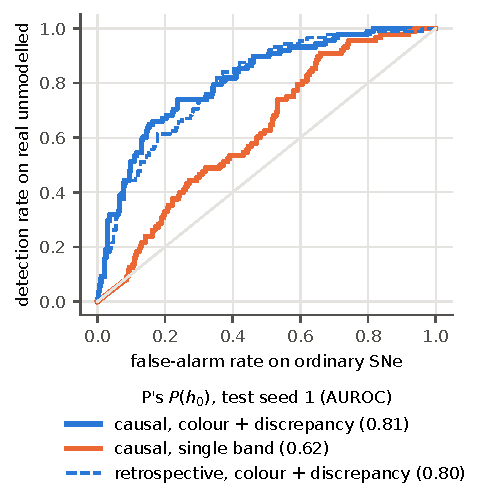
\includegraphics[width=\columnwidth]{generated/figures/fig4_roc_real.pdf}
\caption{Real data: ROC of the open-world planner's $P(h_0)$ for separating real unmodelled transients (TDE, SLSN, SN~Ibn) from ordinary supernovae, test seed 1. Colour plus model discrepancy is what makes $h_0$ usable, and enforcing causality leaves the curve almost unchanged.}
\label{fig:rocreal}
\end{figure}

\paragraph{What causality changed.} The retrospective runs failed H3 and H5. There, P paid for its safety on unknowns with more confident errors and lower accuracy on ordinary supernovae. With causality, H3 passes, the false-``unknown'' rate on supernovae falls from \RealRFaP\ to \RealCFaP, and P's supernova accuracy (\RealCAccModP) matches B3's (\RealCAccModBthree). H5 still fails, but narrowly. On two seeds, the lower confidence bound falls just below $-5$ points, so we cannot rule out a small loss. The cost moved to the unknowns instead: P now flags \RealCFlagP\ of them, against \RealRFlagP\ retrospectively. The reason is the measurement budget. With a time arrow, one-step utilities jump to a late, informative epoch and give up the earlier ones. P used \RealCObsP\ of its 5 measurements on average (B3 \RealCObsBthree, fixed-cadence B0 \RealCObsBzero), against \RealRObsP\ when it could go back in time. Fewer measurements make every posterior less confident, so confident errors drop on both populations, and some of P's detections go with them.

